%!TEX root =../MemoriaTFM.tex
%El anterior comando permite compilar este documento llamando al documento raíz
\chapter{Descripción de la Técnica}\label{chp-02}
\epigraph{A good DevOps organization will free up developers to focus on doing what they do best: write software. }{Rob Steward, 2015\\Global Vicepresident at Verint-Systems}

\lettrine[lraise=-0.1, lines=2, loversize=0.2]{P}{ara} comprender el desarrollo del trabajo aquí presentado, tal y como se ha llevado a cabo, se debe conocer la situación en que éste se desarrolla, la tecnología de la que se dispone y los elementos existentes y necesarios, de una manera objetiva.

Es por esto, que el apartado actual está orientado a conocer las características de la realidad representada y a introducir las bases tecnológicas del presente \gls{TFM}, resaltando los conceptos más importantes.

\section{Metodología ágil}

La tecnología actual avanza a una velocidad considerable, provocando a su paso la renovación de la gestión de proyectos informáticos, debiendo esta alcanzar la velocidad de los cambios ocasionados por esta aceleración. 

Así, la calidad, eficiencia, rapidez y flexibilidad en la entrega de un determinado producto se ha convertido en prioritaria, dando paso a la conocida como metodología ágil.

La metodología ágil envuelve un enfoque para la toma de decisiones en los proyectos software que plantean métodos de ingeniería del software basado en el desarrollo iterativo e incremental, donde los requisitos y las soluciones evolucionan con el tiempo según la necesidad del proyecto. Así el trabajo es realizado mediante la colaboración de equipos auto-organizados y multidisciplinarios, inmersos en un proceso compartido de toma de decisiones a corto plazo\cite{vera2014}.

El uso de procesos ágiles puede reportar los siguientes beneficios a la compañía:

\begin{itemize}
	\item Flexibilidad en el proceso y las definiciones de los productos.
	\item Realimentación continua con el cliente.
	\item Iteracción constante del producto, que se va analizando a medida avanza.
	\item Calidad mejorada.
\end{itemize}

La \autoref{agil} muestra el ciclo de vida en cada iteracción que sufre la aplicación mediante la utilización de dicha metodología.

\begin{figure}[htbp]
	\centering
	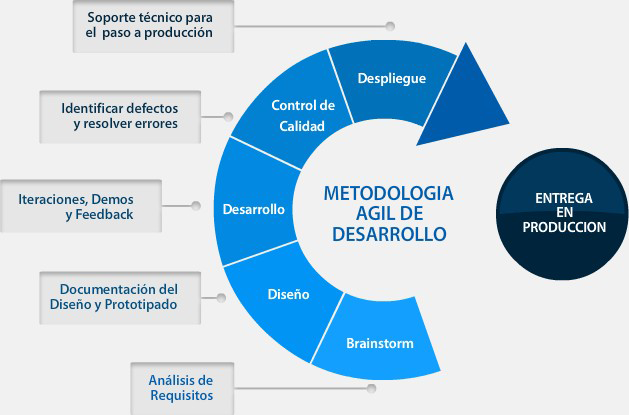
\includegraphics[width=1.0\linewidth]
	{tecnica/figuras/agil.png}
	\caption{CAMBIAR LA IMAGEN}
	\label{agil}
\end{figure}

\section{Integración Continua (\gls{IC}) y Despliegue Continuo (\gls{DC})}

Integración continua (\gls{IC}) es una práctica de desarrollo que requiere que los desarrolladores integren nuevos cambios en el código de la aplicación varias veces en un sólo día. Cada vez que esto ocurre, la inserción es verificada por una compilación automática, permitiendo a los equipos de trabajo implicados en el proceso detectar cualquier problema que el código pudiera contener en cortos periodos de tiempo.

Integrando código regularmente los errores pueden ser detectados rápidamente y corregidos con más facilidad, debido a que se trata de un proceso muy frecuente, la búsqueda del error va a quedar muy acotada.

Por otro lado, el Despliegue Continuo (\gls{DC}) está estrechamente relacionado a la \gls{IC} y está referido a la liberación del código, en los entornos de producción de la compañía, que está sometido a pruebas continuamente y de forma automática.

Adoptar ambos conceptos (\gls{IC} y \gls{DC}) no solo reduce los riesgos y permite una localización temprana de fallos de código, sino que también permite aumentar la velocidad de trabajo con el \gls{SW}\cite{IC2017}.

\section{Ciclo de Desarrollo Seguro de software (\gls{SDLC})}

Un ciclo de Desarrollo Seguro de software (en inglés, Software Development Life Cycle, \gls{SDLC}) es un marco de trabajo que define el proceso utilizado por las compañías a la hora de construir una aplicación desde sus inicios hasta el desmantelamiento de la misma. A lo largo de los últimos años,han surgido multitud de modelos para \gls{SDLC}, que han sido utilizados de diversas maneras acorde a las circunstancias de cada aplicación o empresa en general. Las fases o etapas comunes a todos estos modelos para el Ciclo de Desarrollo de software son las siguientes:

\begin{itemize}
	\item Requisitos y planificación.
	\item Arquitectura y diseño.
	\item Planificación de las pruebas.
	\item Desarrollo del código.
	\item Pruebas y resultados.
	\item Lanzamiento y mantenimiento.
\end{itemize}

Con esto, un proceso de implementación de seguridad en el proceso \gls{SDLC} garantizará que las actividades de seguridad, como las pruebas de penetración, la revisión del código y el análisis de la arquitectura, son parte integral del esfuerzo de desarrollo.

\section{Análisis estático}

Análisis estático, o también conocido por análisis estático de código, es un método de depuración de aplicaciones que se basa en exámenes al código cuando éste no se está ejecutando. El proceso de análisis estático es realizado con la ayuda de herramientas automatizadas y asiste a los desarrolladores aportando valiosa información mediante el escrutinio del código, utilizando mecanismos y herramientas (por ejemplo revisión de impresiones y campos de formularios) que podrían escapar al ojo humano\footnote{El análisis realizado por un humano recibe el nombre de comprensión de código}\cite{rouse2017}.

\section{Dependencias de software}\label{dependencias}

En el campo de la programación y el software una dependencia de código o \gls{SW} es una aplicación o biblioteca de código requerida por otro programa para poder funcionar de manera correcta\cite{wiki2017}.

La lista de dependencias de \gls{SW} que una aplicación ruby o una aplicación escrita con el lenguaje de programación node van a requerir se almacenan en archivos específicos llamados Gemfile.lock y package.json, respectivamente. 

\section{Virtualización basada en contenedores}

La nube es cada vez más grande, más potente y posee más usuarios. Al mismo tiempo, permite la ejecución de aplicaciones más y más potentes, que requieren garantizar el correcto funcionamiento de esta, actualmente y en el futuro.

Por este motivo, es primordial utilizar una plataforma que optimice los recursos, en la medida de lo posible, a la vez que permita la escalabilidad, con el fin de poder ampliar sus características de forma sencilla en caso de ser necesario.

Al hablar de nube se está hablando de virtualización. Ejecutar un \gls{SO} virtual para cada instancia de una aplicación es un proceso muy pesado y lento, es de este problema donde surge el concepto de virtualización basada en contenedores, también conocida como virtualización a nivel de sistema operativo.

Un contenedor no es más que una nueva forma de optimizar los recursos de los que dispone una plataforma, creando pequeños espacios virtuales de las aplicaciones necesarias, en las que unicamente se tendrá que cargar el núcleo de la aplicación y las dependencias de esta, pero funcionando siempre sobre un único kernel, o sitema operativo\cite{velazco2016}. La \autoref{contenedores} muestra las diferencias en el modelo de capas de un sistema de virtualización tradicional y uno basado en contenedores.

\begin{figure}[htbp]
	\centering
	\includegraphics[width=0.8\linewidth]
	{tecnica/figuras/Contenedores.png}
	\caption{Sistemas de vitualización}
	\label{contenedores}
\end{figure}

\endinput